\section{Ergo's Native Token}
\label{sec:currency}

Ergo platform has its native token, which is
called \Erg{} and is divisible to up to $10^9$ smallest units, \nanoErg{}s~(a \nanoErg{} is one billionth of an Erg).
\Erg{}s are important for Ergo platform stability and security by several reasons discussed below.

During the initial phase of Ergo's life, miners will receive the reward in \Erg{}s
according to a predefined and hard-coded token emission schedule~(see~\ref{sec:emission} for more details).
These coins will incentivize miners to participate in the Ergo network, securing it from hashrate-based attacks
like the known 51\% attack~\cite{reorgAttack}.

\Erg{} emission will be finished within just eight years, and after that miners will only receive \Erg{}s from
fees.
Although, adjustable over time through miner on-chain voting, Ergo block size and maximum block computational
cost at any given point in time will be limited,
and thus miners are enforced to
choose only a subset of transactions from mempool during times of high load.
Fees will help miners to sort the transactions, preventing spam attacks while allowing miners
to include transactions from honest users in blocks.

Besides network and computation resources, a transaction utilizes storage by increasing state size.
In existing cryptocurrencies, an element of the state, being  a UTXO  in  UTXO-based  blockchains,  called  a box
in  Ergo, once created lives possibly forever without any compensation to miners and some users who must keep this state
in high-cost random-access memory. This leads to a misalignment of incentives and continuously increasing state size.
In contrast, Ergo has a storage rent component that periodically charges users Erg for every byte
included in the state.
This storage rent is making the system more stable by limiting state size or insuring proper compensation for larger
state size, returning lost coins into
circulation and providing an additional stable and predictable reward to miners.

Thus, being a platform for contractual money, Ergo is suitable to build applications and monetary systems
on top of it.
However, participating in such systems would require using the Ergo native token, Erg, as well in order to pay
storage rent and transaction fees which will provide miners strong ongoing incentives to secure the network with
adequate hash power. Users, for their part, will be highly incentivized to purchase, use and save Ergs if they
find applications for Ergo to be of high value.

\subsection{Emission}
\label{sec:emission}


All \Erg{} tokens that will ever circulate in the system are presented in the initial state, which consists of 3 boxes:

\begin{itemize}
    \item{\em No Premine Proof.} This box contains exactly one~\Erg{} and is protected by a script that prevents it from being spent by anyone.
    Thus, it is a long-lived box that will stay in the system until the storage-rent component
    destroys it.
    Its main purpose is to prove that \Ergo{} mining was not started privately by anyone before
    the declared launch date.
    To achieve this, additional registers of this box contain the latest headlines from the media (The Guardian, Vedomosti, Xinhua), as well as the latest block identifiers from Bitcoin and Ethereum.
    Thus, \Ergo{} mining could not have started before certain events in the real world and the cryptocurrency space.

    \item{\em Treasury.} This box contains 4,330,791.5 \Erg{}s that will be used to fund \Ergo{}
    development.
    Its protecting script~\cite{scriptTreasury} consists of two parts.

    First, it ensures that only a predefined portion of the box value is unlocked.
    During blocks 1-525,599 (2 years) 7.5 \Erg{}s will be released every block. Then during blocks 525,600-590,399 (3 months) 4.5 \Erg{}s will be released every block. Finally,
    during blocks 590,400-655,199 (3 months) 1.5 \Erg{}s will be released every block.
    This rule ensures the presence of funds for \Ergo{} development for 2.5 years and, at any moment of time,
    rewards do not exceed 10\% of the total number of coins in circulation.

    Second, it has custom protection from unexpected spending.
    Initially, it requires the spending transaction to be signed by at least 2 of 3 secret keys that are under control of the initial team members. When they spend the box, they are free to
    change this part of the script as they wish, for example by adding new members to protect foundation
    funds.

    During the first year, these funds will be used to cover the pre-issued EFYT token%~\cite{our website with swap }
. After that, they will be distributed in a decentralized manner via a community voting system that is under development.


    \item{\em Miners Reward.} This box contains 93,409,132 \Erg{}s that will be collected by block miners
    as a reward for their work.
    Its protecting script~\cite{scriptEmission} requires the spending transaction to have exactly two outputs with the following properties:

    \begin{itemize}
    \item{} The first output should be protected by the same script and the number of \Erg{}s in it should
    equal to the remaining miners' reward.
    During blocks 1 - 655,199, a miner will be able to collect 67.5 \Erg{}s from this box. During blocks 655,200 - 719,999 (3 months), a miner will be able to collect 66 \Erg{}s, and after that, the block reward will be reduced by 3 \Erg{}s every 64,800 blocks (3 months) until it reaches zero at block 2,080,800.

    \item{} The second output should contain the remaining coins and should be protected by the following condition:
    it can be spent by a miner that solved the block's PoW puzzle and not earlier than 720 blocks after the current block.
    \end{itemize}

\end{itemize}

All of these rules result in the following curve denoting the number of coins in circulation with time:

\begin{figure}[H]
    \centering
    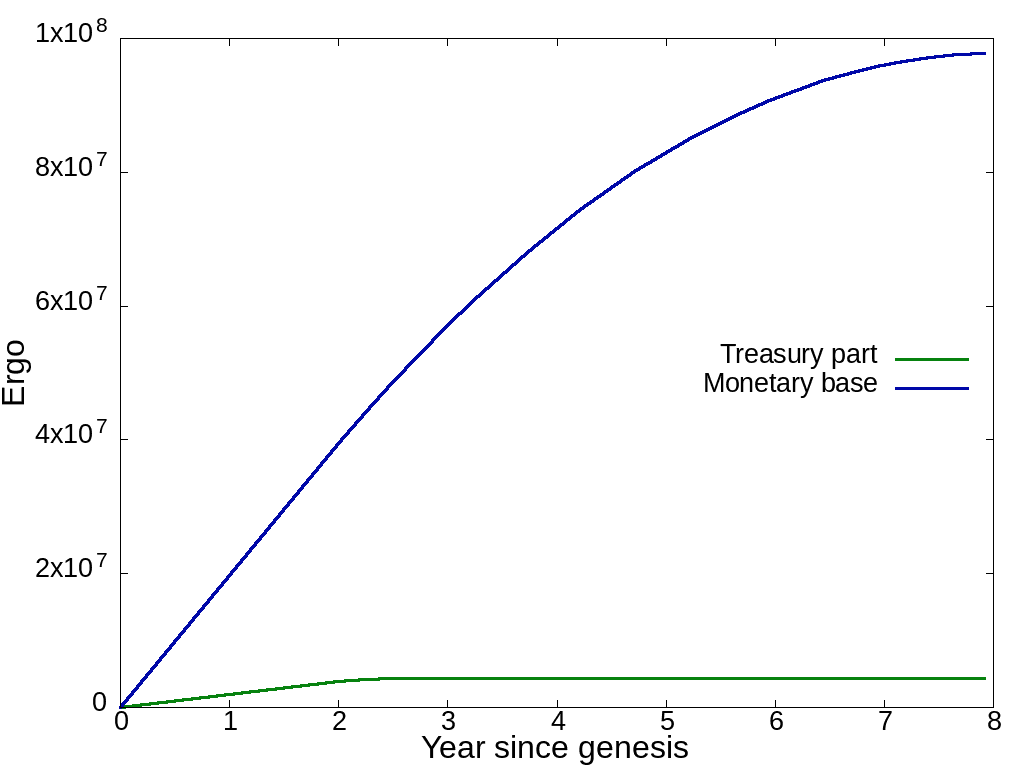
\includegraphics[width=\textwidth]{img/emission.png}
    \caption{Ergo emission curve
    \label{fig:emission} }
\end{figure}
